%\section{Serializador e Deserializador disponíveis na FPGA}
%
%As FPGA de série 7 da XILINX têm disponíveis transcetores capazes de comunicação em série de alta velocidade, tal como é necessário neste projeto. Em específico, na FPGA XILINX VC7203 Virtex-7 estão disponíveis transcetores GTX que permitem uma velocidade de 10 Gb/s e que são os mais adequados para conexão à fibra ótica. Noutros modelos existem outros transcetores, como por exemplo GTZ (que permite até 28 Gb/s), GTH (que permite débitos até 13,1 Gb/s) e GTP (com débitos até 6,6 Gb/s). No entanto apenas serão abordados os transcetores GTX, visto que são os mais adequados para este tipo de comunicações.
%
%\begin{figure}[h!]
%	\begin{center}
%		\leavevmode
%		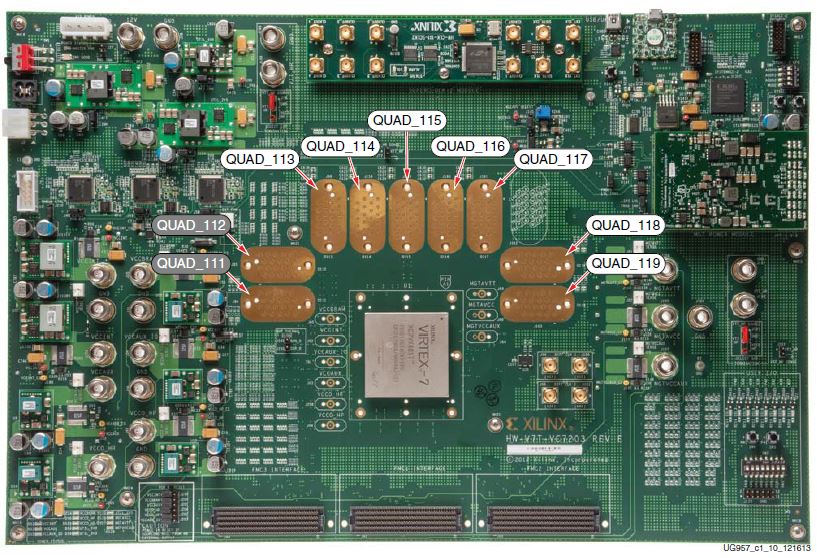
\includegraphics[width=1.0\textwidth]{gtxLOCA}
%		\caption{Identificação dos transcetores GTX na FPGA VC7203 Virtex-7, retirada de \cite{R008}}
%		\label{fig:GTXlocalização}
%	\end{center}
%\end{figure}
%
%Na figura~\ref{fig:GTXlocalização} na página~\pageref{fig:GTXlocalização} é possível visualizar a FPGA a ser utilizada no projeto e visualiza-se ainda assinaladas as entradas GTX (QUAD\_111, QUAD\_112, QUAD\_113, QUAD\_114, QUAD\_115, QUAD\_116, QUAD\_117, QUAD\_118 e QUAD\_119). 
%Os transcetores baseiam-se na seguinte arquitetura, segundo \cite{R010}:
%\begin{itemize}
%	\item \textbf{PMA (\textit{Physical Medium Attachment Sublayer})} que inclui:
%	\begin{itemize}
%		\item suporte de taxas de débito até 12,5 Gb/s
%		\item uma PLL por canal para melhor flexibilidade do sinal de relógio
%		\item uma interface que faz a conversão de série para paralelo e de paralelo para série (PISO e SIPO)
%		\item uma PLL (\textit{Phase-Locked Loop})
%		\item Equalizador de decisão com feedback (DFE)
%		\item CDR (\textit{clock data recovery})
%		\item Bloco de pré-ênfase e equalização
%		\item Saída do transmissor programável
%	\end{itemize}
%	\item \textbf{PCS (\textit{Physical Coding Sublayer}) que inclui:}
%	\begin{itemize}
%		\item \textit{Datapath} de 2 e 4 byte internos para suportar diferentes taxas de débitos
%		\item Codificação e descodificação 8B/10B
%		\item Deteção de vírgula e alinhamento de palavra
%		\item PRBS (\textit{Pseudo Random Bit Sequence}) gerador e verificador
%		\item FIFO para correção do sinal de relógio e ligação do canal
%		\item Lógica que processa os dados em paralelo reconfigurável
%		\item Este bloco trabalha com taxas de débitos de informação mais baixas.
%	\end{itemize}
%\end{itemize}
%
%É possível visualizar um diagrama geral da arquitetura dos transcetores GTX disponíveis na FPGA na figura~\ref{fig:GTXarquitetura} na página~\pageref{fig:GTXarquitetura}.
%
%\begin{figure}[h!]
%	\begin{center}
%		\leavevmode
%		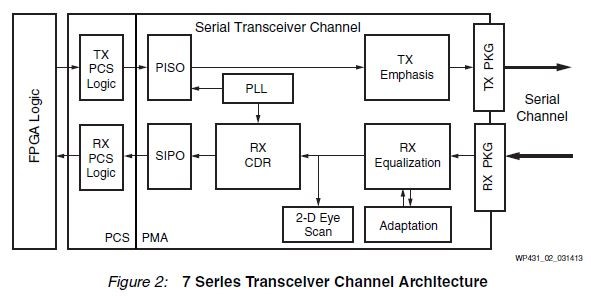
\includegraphics[width=1.0\textwidth]{gtxAqr}
%		\caption{Arquitetura geral dos transcetores GTX, retirada de \cite{R010}}
%		\label{fig:GTXarquitetura}
%	\end{center}
%\end{figure}
%
%O transmissor e o recetor passam a ser descritos mais detalhadamente de seguida.

\subsubsection{Transmissor}
Cada transcetor GTX inclui um transmissor independente que consiste num módulo PCS e um modulo PMA, tal como referido anteriormente. A figura~\ref{fig:gtx_tx} na página~\pageref{fig:gtx_tx} representa o diagrama de blocos do transmissor.
\begin{figure}[h!]
	\begin{center}
		\leavevmode
		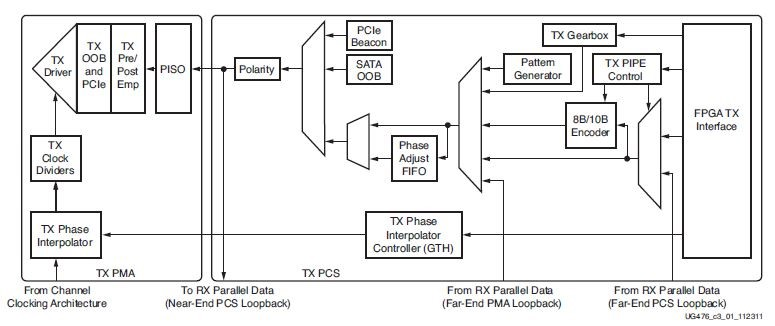
\includegraphics[width=1.0\textwidth]{gtx_tx}
		\caption{Diagrama de blocos de um transmissor GTX, retirada de \cite{R011}}
		\label{fig:gtx_tx}
	\end{center}
\end{figure}

Os dados provenientes da FPGA, cujo formato é em paralelo, passam para a interface transmissora, de seguida para os módulos PCS e PMA e, por fim, para a saída pelo driver do transmissor a alta velocidade. 

O transmissor contém os seguintes blocos principais, cujas funcionalidades passam a ser brevemente resumidas, segundo \cite{R010}:
\begin{enumerate}
	

	\item \textbf{Interface transmissora da FPGA}
	
	\hspace{1.0em}Esta interface serve como porta de comunicação entre a FPGA e o datapath do transmissor. Esta comunicação é feita através da escrita de dados na porta TXDATA na transição de 0 para 1 do sinal de relógio TXUSRCLK2.
	
	\hspace{1.0em}O tamanho do sinal a ser transmitido pode ser configurado para 2, 4 ou 8 bytes. Na realidade este tamanho é definido por TX\_DATA\_WIDTH e TX\_INT\_DATAWIDTH e ainda por TX8B19BEN, e o tamanho interno destes sinais pode ser 16, 20, 32, 40, 64 e 80 bits. A tabela~\ref{table:dataTXDATA} na página~\pageref{table:dataTXDATA} demonstra como esses tamanhos são configurados através das entradas referidas.
	
% Please add the following required packages to your document preamble:
% \usepackage{multirow}
\begin{table}[]
	\centering
	\begin{tabular}{|c|c|c|c|c|}
		\hline
		\textbf{TX8B10BEN} & \textbf{TX\_DATA\_WIDTH} & \textbf{TX\_INT\_DATAWIDTH} & \textbf{\begin{tabular}[c]{@{}c@{}}Tamanho na interface \\ da FPGA (bits)\end{tabular}} & \textbf{\begin{tabular}[c]{@{}c@{}}Tamanho interno \\ dos dados (bits)\end{tabular}} \\ \hline
		\multirow{4}{*}{1} & 20                       & 0                           & 16                                                                                      & 20                                                                                   \\ \cline{2-5} 
		& 40                       & 0                           & 32                                                                                      & 20                                                                                   \\ \cline{2-5} 
		& 40                       & 1                           & 32                                                                                      & 40                                                                                   \\ \cline{2-5} 
		& 80                       & 1                           & 64                                                                                      & 40                                                                                   \\ \hline
		\multirow{8}{*}{0} & 16                       & 0                           & 16                                                                                      & 16                                                                                   \\ \cline{2-5} 
		& 20                       & 0                           & 20                                                                                      & 20                                                                                   \\ \cline{2-5} 
		& 32                       & 0                           & 32                                                                                      & 16                                                                                   \\ \cline{2-5} 
		& 32                       & 1                           & 32                                                                                      & 32                                                                                   \\ \cline{2-5} 
		& 40                       & 0                           & 40                                                                                      & 20                                                                                   \\ \cline{2-5} 
		& 40                       & 1                           & 40                                                                                      & 40                                                                                   \\ \cline{2-5} 
		& 64                       & 1                           & 64                                                                                      & 32                                                                                   \\ \cline{2-5} 
		& 80                       & 1                           & 80                                                                                      & 40                                                                                   \\ \hline
	\end{tabular}
	\caption{Configuração do tamanho dos dados de TXDATA, adaptada de \cite{R011}}
	\label{table:dataTXDATA}
\end{table}

	\hspace{1.0em}Quando o codificador 8B/10B está ativo, então TX\_DATA\_WIDTH deve estar configurado para 20, 40 ou 80 bits e nesta situação, a interface do transmissor com a FPGA apenas utiliza os dados provenientes da porta TX\_DATA\_WIDTH. Quando o mesmo está desativo, então TX\_DATA\_WIDTH pode estar configurado para 16,20,32,40,64 ou 80 bits.

	\hspace{1.0em}O sinal TX\_INT\_DATAWITH é um atributo que configura a ativação do datapath de 2 e 4 bytes disponível internamente no transcetor.

	\hspace{1.0em}Para além do sinal de relógio TXUSRCLK2, que é o sinal de relógio principal para a sincronização dos sinais que chegam ao transmissor, existe um segundo sinal de relógio paralelo que é usado internamente para operações lógicas a realizar no módulo PCS. Este segundo sinal de relógio, TXUSRCLK, irá depender do tamanho interno dos dados usado no datapath e da taxa de transmissão do transmissor GTX. É possível calcular esta mesma taxa através da divisão entre a taxa de transmissão da linha e do tamanho interno dos dados utilizado no datapath. Para além disso, estes dois sinais de relógio têm uma relação fixa que determina os seus valores que depende dos valores presentes em TX\_DATA\_WIDTH e TX\_INT\_DATAWIDTH. Essas relações estão apresentadas na tabela~\ref{table:freqTXgtx} na página~\pageref{table:freqTXgtx}:

\begin{table}[]
	\centering
	\begin{tabular}{|c|c|c|c|}
		\hline
		\textbf{\begin{tabular}[c]{@{}c@{}}Tamanho na \\ interface da\\  FPGA (byte)\end{tabular}} & \textbf{TX\_DATA\_WIDTH} & \textbf{TX\_INT\_DATAWIDTH} & \textbf{Frequência de TXUSRCLK2} \\ \hline
		2                                                                                          & 16, 20                   & 0                           & f(TXUSRCLK2) = f(TXUSRCLK)       \\ \hline
		4                                                                                          & 32, 40                   & 0                           & f(TXUSRCLK2) = f(TXUSRCLK) / 2   \\ \hline
		4                                                                                          & 32, 40                   & 1                           & f(TXUSRCLK2) = f(TXUSRCLK)       \\ \hline
		8                                                                                          & 64, 80                   & 1                           & f(TXUSRCLK2) = f(TXUSRCLK) / 2   \\ \hline
	\end{tabular}
	\caption{Configuração da frequência de TXUSRCLK2, adaptada de \cite{R011}}
	\label{table:freqTXgtx}
\end{table}

	\hspace{1.0em}Assim sendo, é possível fazer uso dos transcetores disponíveis na FPGA, utilizando um tamanho adequado de dados para a transmissão, tendo em conta as configurações necessárias e disponíveis para tal, tal como descrito anteriormente. Por outras palavras, utilizando tamanhos de entradas devidamente apropriados, será fácil enviar os dados recebidos e descodificados do HDMI através destes transcetores, que pode vir a ser útil numa fase inicial do projeto.

	\item \textbf{Codificador 8B/10B do transmissor}
	
	\hspace{1.0em}Esta é a codificação utilizada no sinal para de seguida fazê-lo enviar pelas portas de alta velocidade, e é uma codificação \textit{standard} que troca dois bits por byte para alcançar um equilíbrio e obter uma disparidade limitada para que a recuperação de relógio seja razoável. O transmissor possui um \textit{datapath} específico para fazer este tipo de codificação e ao mesmo tempo poupar recursos da FPGA apesar de aumentar a latência no caminho do transmissor.
	
	\hspace{1.0em}A ativação ou não deste bloco é representada no sinal TX8B10BEN. Quando está ativo, o sinal passado na interface do transmissor com a FPGA por TXDATA é codificado antes de ser enviado pelas saídas de alta velocidade, caso contrário, tal não acontece e o sinal é enviado tal como é transmitido. 
	
	\item \textbf{\textit{Gearbox} do transmissor}
	
	\hspace{1.0em}Este bloco suporta a codificação do sinal 64B/66B e 64B/67B, uma vez que este tipo de codificação é utilizada em alguns protocolos de comunicação de alta velocidade. Esta utilização permite reduzir a sobrecarga da codificação 8B/10B e ao mesmo tempo reter os benefícios de um esquema de codificação. Este bloco suporta interfaces de 2, 4 ou 8 bytes e a codificação dos dados é feita na lógica da FPGA. 
	
	\item \textbf{\textit{Buffer} do transmissor}
	
	\hspace{1.0em}O transmissor GTX tem disponível também um buffer e um bloco de alinhamento de fase no seu circuito para que possa sincronizar os diferentes domínios dos sinais de relógio. Isto acontece porque internamente o transmissor tem dois sinais de relógios paralelos: o sinal do domínio PMA (XCLK) e o sinal de relógio TXUSRCLK. No entanto, quando a transmissão de dados entre estes dois domínios é realizada é necessário que os sinais estejam sincronizados e as diferenças de fase resolvidas. Como tal, será necessário a utilização deste bloco para se poder realizar a sincronização entre os sinais.
	
	\hspace{1.0em}O circuito de alinhamento da fase é utilizado para resolver a diferença entre as fases dos sinais quando o buffer não está ativo. Mas pelo menos um dos blocos deve ser sempre utilizado. 
	
	\hspace{1.0em}A utilização do \textit{buffer} é mais fácil e é sempre recomendada a sua utilização, enquanto que o bloco de alinhamento de fase é um bloco mais complexo no que toca a lógica e que requer restrições adicionais nas fontes dos sinais de relógio. Por outro lado, o buffer não deve ser utilizado quando a latência é uma questão importante do circuito, uma vez que o bloco de alinhamento de fase consegue alcançar menor latência. 
	
	\item \textbf{Gerador de padrões do transmissor} 
	
	\hspace{1.0em}A geração de sequência pseudoaleatórias é bastante utilizada em sistemas de telecomunicações para testar a integridade do sinal de ligações de grande velocidade. Apesar de estas mesmas sequências parecerem aleatórias à primeira vista, na realidade apresentam determinadas características que são utilizadas para medir a qualidade da ligação. Este bloco do transmissor é responsável por esta ação. 
	
	\item \textbf{Controlo de polaridade do transmissor} 
	
	\hspace{1.0em}Este bloco é responsável por inverter os dados em paralelo antes da sua serialização e transmissão para compensar a inversão de polaridade no par diferencial, isto porque tal pode levar a uma inversão de polarização dos dados transmitidos pelo GTX quando TXN e TXP são acidentalmente trocados na PCB. 
	
	\item \textbf{Controlo do sinal de relógio de saída do transmissor}
	
	\hspace{1.0em}Este bloco é responsável pelo controlo da divisão do sinal de relógio em série e pelo controlo da divisão e seleção do sinal de relógio em paralelo.
	
	\hspace{1.0em}No que toca à divisão do sinal de relógio em série, cada módulo PMA do transmissor possui um divisor D que divide o sinal de relógio da PLL para suportar taxas de transmissão mais baixas. Este divisor pode ser definido estaticamente para aplicações com uma taxa de transmissão fixa, mas também pode ser utilizado para ligações onde a taxa de transmissão pode variar e como tal D varia com essa mesma variação. Este bloco é responsável por esta divisão do sinal de relógio em série. 
	
	\hspace{1.0em}Quanto à divisão e seleção do sinal de relógio paralelo, o sinal de relógio em paralelo que sai deste bloco de controlo de divisão de relógio pode ser utlizado como o relógio de fabrico lógico, dependendo das linhas de transmissão requisitadas. Este bloco controla também essa mesma divisão e seleção.
	
	\item \textbf{Driver reconfigurável do transmissor}
	
	\hspace{1.0em}É um \textit{buffer} de saída diferencial de alta velocidade que possui características para maximizar a integridade do sinal, tal como controlo diferencial de tensão, pré-ênfase e resistências de terminação calibradas.
	
	\item \textbf{Suporte de deteção de recetor para arquiteturas \textit{PCI Express}}
	
	\hspace{1.0em}As especificações das arquiteturas PCI Express incluem características que permitem detetar a presença do recetor para uma determinada ligação. Este bloco é responsável por esta mesma deteção.	
\end{enumerate}

\subsubsection{Recetor}

Cada transcetor possui um recetor independente, cujo diagrama de blocos está representado na figura~\ref{fig:gtx_rx} na página~\pageref{fig:gtx_rx}. Mais uma vez, o recetor possui dois módulos principais: PCS e PMA. 

O sinal de alta velocidade em série chega ao RX ao modulo PMA, passa por PCS e, por fim, passa para a lógica da FPGA pela interface com a mesma.

\begin{figure}[h!]
	\begin{center}
		\leavevmode
		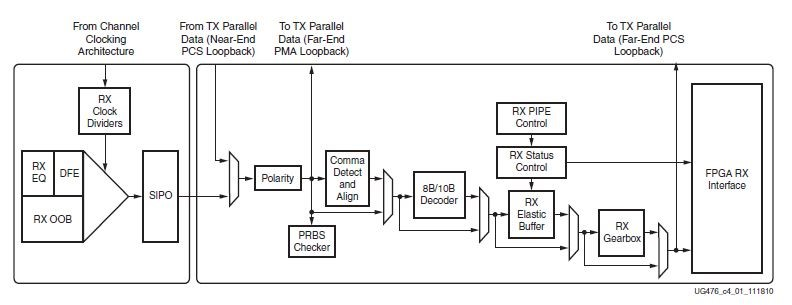
\includegraphics[width=1.0\textwidth]{gtx_rx}
		\caption{Diagrama de blocos de um recetor GTX, retirada de \cite{R011}}
		\label{fig:gtx_rx}
	\end{center}
\end{figure}

É possível dividir o recetor GTX nos seguintes principais blocos que passam brevemente a ser descritos:

\begin{enumerate}
	\item \textbf{\textit{Front End} Analógico do recetor}
	
	\hspace{1.0em}É um buffer diferencial de entrada de modo de corrente de alta velocidade que possui determinadas características tais como: reconfiguração de tensão de terminação do recetor e calibração das resistências de terminação.
	
	\item \textbf{Equalizador do recetor}
	
	\hspace{1.0em}Ao longo da transmissão, diversos erros podem acontecer nos dados transmitidos e, como tal, são necessários filtros que permitam ou que pelo menos ajudem a realizar a recuperação do sinal recebido corretamente. Os transcetores GTX disponibilizam filtros adaptativos para tal recuperação: LPM que está otimizado para canais com poucas perdas e ainda DFE para canais com perdas maiores. As arquiteturas apresentadas de seguida foram arquiteturas brevemente abordadas anteriormente dentro deste capítulo que estão referidas em \cite{R012}.
	
	\hspace{1.0em}Na figura~\ref{fig:eq_LPM} na página~\pageref{fig:eq_LPM} encontra-se o diagrama de blocos do equalizador LPM. Este modo é recomendado para aplicações com débitos até 11,2 Gb/s de curto alcance, com perdas de canal até 12 dB à frequência de Nyquist.
	
	\begin{figure}[h!]
		\begin{center}
			\leavevmode
			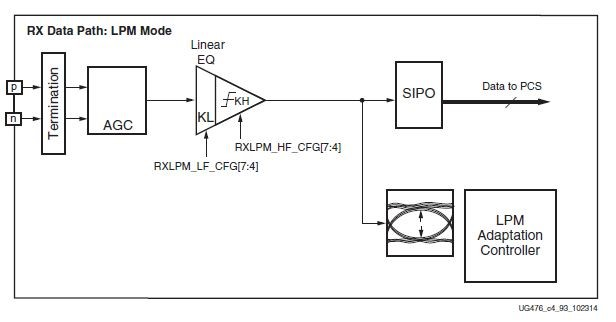
\includegraphics[width=1.0\textwidth]{equalizador_LPM}
			\caption{Equalizador em modo LPM, retirada de \cite{R011}}
			\label{fig:eq_LPM}
		\end{center}
	\end{figure}

	\hspace{1.0em}Na figura~\ref{fig:eq_DFE} na página~\pageref{fig:eq_DFE} é possível visualizar o diagrama de blocos utilizado para o equalizador DFE (Decision Feedback Equalizer). Este é um filtro que utiliza a realimentação de símbolos detetados para produzir uma estimação da saída do canal. O DFE é alimentado com os símbolos já detetados e produz uma saída que é a combinação da saída do equalizador linear com estes mesmo símbolos já detetados.  

	\begin{figure}[h!]
	\begin{center}
		\leavevmode
		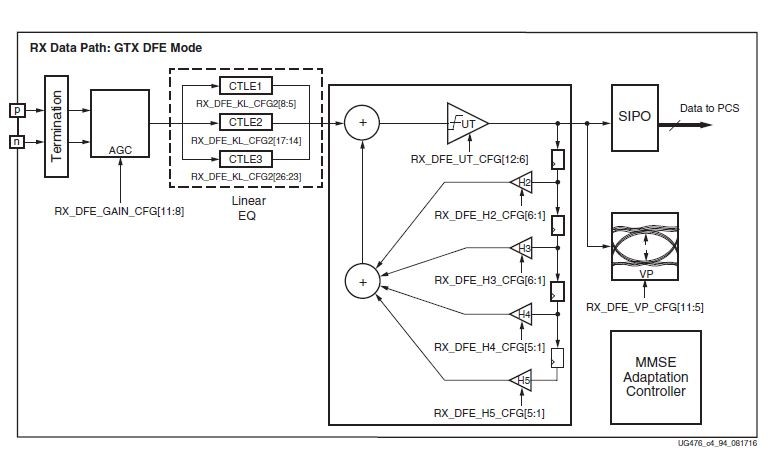
\includegraphics[width=1.0\textwidth]{equalizador_DFE}
		\caption{Equalizador em modo DFE, retirada de \cite{R011}}
		\label{fig:eq_DFE}
	\end{center}
	\end{figure}	

	\hspace{1.0em}Este equalizador é utilizado para ligações de média distância cujas perdas do canal rondam os 8 dB ou mais à frequência de Nyquist. 
	
	\hspace{1.0em}\textbf{Vantagens da utilização deste tipo de equalizador:}
	\begin{itemize}
		\item Efetua a equalização sem amplificação do ruído ou interferência
		\item Pode também fazer correções de reflexões causadas pelas descontinuidades do canal 
		\item É vantajosa a sua utilização quando as interferências são preocupantes 
	\end{itemize}
	
	\hspace{1.0em}\textbf{Cuidados a ter na utilização deste tipo de equalizador:}
	\begin{itemize}
		\item Este tipo de equalização deve ser cuidadosa quando não existe codificação de dados, uma vez que pode levar à não equalização ideal do sinal recebido (pois o filtro pode não se auto adaptar aos dados recebidos).
	\end{itemize}

	\hspace{1.0em}Visto que neste projeto se pretende realizar comunicações de média/longa distância, deve ser utilizado o equalizador DFE para obter uma boa equalização do sinal recebido. 
	
	\item \textbf{CDR (\textit{Clock Data Recovery}) do recetor}
	
	\hspace{1.0em}O circuito de CDR faz a recuperação do relógio dos dados recebidos em série. Na figura~\ref{fig:cdr} na página~\pageref{fig:cdr} é possível encontrar a arquitetura deste mesmo circuito. Este circuito foi também já brevemente referido no subcapítulo anterior que refere as considerações a tomar quando se implementam arquiteturas de serialização e deserialização, e passa de seguida a ser descrito.
	
	\begin{figure}[h!]
		\begin{center}
			\leavevmode
			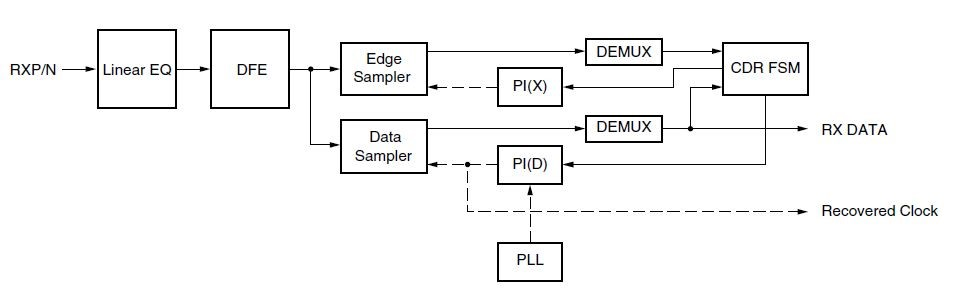
\includegraphics[width=1.0\textwidth]{CDR}
			\caption{Detalhes do circuito CDR (\textit{Clock data recovery}), retirada de \cite{R011}}
			\label{fig:cdr}
		\end{center}
	\end{figure}

	\hspace{1.0em}A tracejado encontra-se o caminho feito pelo sinal de relógio até à sua recuperação. 
	Os dados recebidos passam pelo equalizador e de seguida são capturados por um “data sampler” e um “edge sampler”. O “edge sampler” captura a fase do sinal recebido em série quando este está na sua região de transição, enquanto que o “data sampler” captura a fase do mesmo sinal a meio do olho dos dados. Estas duas fases são de seguida enviadas para a máquina de estados do CDR para que esta consiga determinar a fase dos sinais que chegam e ao mesmo tempo controlar os interpoladores de fase (PIs).
	
	\item \textbf{Controlo do sinal de relógio de saída} 
	
	Tal como no transmissor, o bloco de divisão de sinal de relógio tem dois principais componentes: controlo da divisão do sinal de relógio em série e ainda controlo e seleção da divisão do sinal relógio em paralelo. As suas funções são iguais à do transmissor.
	
	\item \textbf{Análise de Margem do Recetor}
	
	\hspace{1.0em}Com o aumento das taxas de débito da transmissão e também da atenuação os equalizadores dos recetores têm mais capacidade de superar a atenuação do canal. Contudo, isto traz um novo desafio, pois nestes casos, a qualidade da ligação não pode ser medida através da abertura do olho no diagrama de olho resultante. 
	
	\hspace{1.0em}Para taxas de transmissão muito altas pode acontecer que o diagrama de olho do sinal recebido possa parecer completamente fechado, apesar de que após a equalização esteja aberto. Como tal, esta medida de qualificação da qualidade da ligação realizada pode então ter de ser reavaliada.
	
	\hspace{1.0em}Assim sendo, os transmissores GTX possuem um mecanismo que permite medir e visualizar a margem do diagrama de olho recebido após equalização. Também existem modos que permitem determinar e diagnosticar os efeitos das configurações de equalização.
	
	\hspace{1.0em}Este mecanismo permite que uma correta avaliação da qualidade do canal e para além disso, pode ser feita enquanto os dados estão a ser recebidos, devido ao seu mecanismo que assim o permite, não exigindo nenhuma alteração às configurações do recetor e nem nenhuma lógica extra da FPGA. 
	
	\item \textbf{Controlo da polarização do recetor}
	
	\hspace{1.0em}Tal como foi mencionado aquando a referência da funcionalidade deste mesmo bloco no transmissor, os sinais RXN e RXP podem ser trocados acidentalmente na PCB e como tal os dados diferencias recebidos pelo recetor estão invertidos. Este bloco é responsável pela inversão dos bytes em paralelo no módulo PCS antes da deserialização do sinal (SIPO) para compensar a polarização inversa do par diferencial.
	
	\item \textbf{Verificador de Padrões do recetor}
	
	\hspace{1.0em}Este bloco é responsável pela verificação de determinados padrões PSBR e faz esta mesma verificação antes do alinhamento das palavras ou descodificação. Tal como descrito aquando a referência ao gerador destes mesmos padrões no transmissor, estes servem para verificar a integridade do sinal na ligação.
	
	\item \textbf{Alinhamento de \textit{Byte} e palavras do recetor}
	
	\hspace{1.0em}Os dados em série que chegam ao recetor devem ser alinhados com limitações de símbolos antes de poderem ser utilizados como dados em paralelo. Assim sendo, o transmissor envia sequências reconhecíveis (normalmente são chamadas de vírgulas) e o recetor procura essa mesma sequência nos dados recebido. Quando a encontra move-a para os limites das palavras para que as palavras em paralelo recebidas sejam iguais às palavras enviadas pelo transmissor. Para ativar a utilização deste bloco o sinal de entrada RXCOMMADETEN deve ser verdadeiro, mas caso a latência seja um parâmetro critico do circuito então este bloco não deve estar ativo. 
	
	\hspace{1.0em}Para definir a sequência que o bloco de alinhamento deve procurar (a vírgula) nos dados que chegam em série ao recetor, então deve-se definir as entradas ALIGB\_MCOMMA\_VALUE, ALIGN\_PCOMMA\_VALUE e ALIGN\_COMMA\_ENABLE. Os tamanhos destas sequências dependerão dos valores em RX\_DATA\_WIDTH, que será explicado mais à frente neste relatório.
	
	\begin{figure}[h!]
		\begin{center}
			\leavevmode
			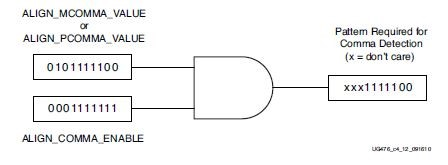
\includegraphics[width=0.7\textwidth]{commaObtain1}
			\caption{Mecanismo de obtenção da “vírgula”, retirado de \cite{R011}}
			\label{fig:comma1}
		\end{center}
	\end{figure}
	
	\hspace{1.0em}A figura~\ref{fig:comma1} na página~\pageref{fig:comma1} ilustra o mecanismo utlizado para obter a sequência de procura dos dados recebidos no recetor quando ALIGN\_COMMA\_DOUBLE é falso. Quando este mesmo sinal é verdadeiro faz-se então uma extensão do sinal ALIGN\_MCOMMA\_VALUE e do sinal ALIGN\_PCOMMA\_VALUE, tal como está representado na figura~\ref{fig:comma2} na página \pageref{fig:comma2}.
	
		\begin{figure}[h!]
		\begin{center}
			\leavevmode
			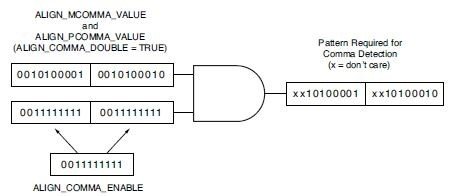
\includegraphics[width=0.7\textwidth]{commaObtain2}
			\caption{Mecanismo de obtenção da “vírgula” quando ALIGN\_COMMA\_DOUBLE=1, retirado de \cite{R011}}
			\label{fig:comma2}
		\end{center}
	\end{figure}
	
	\hspace{1.0em}Quando este mesmo sinal está ativo os sinais de entrada ALIGN\_MCOMMA\_VALUE e ALIGN\_PCOMMA\_VALUE são combinados e o bloco procura por duas sequências de uma vez nos mesmos dados recebidos. Para ativar o alinhamento de palavras da sequência MCOMMA o sinal RXMCOMMAALIGNEN deve estar ativo, enquanto que para ativar o alinhamento da palavra PCOMMA o sinal RXPCOMMAALIGNEN deve estar ativo. Quando ambas estão ativas então o alinhamento é realizado com qualquer padrão.
	
	\hspace{1.0em}É necessário ter em atenção que em aplicações cuja taxa de débito é superior a 5 Gb/s e que têm demasiado ruído, pode acontecer por vezes um falso alinhamento de palavras que leva à ativação do sinal. Isto indica que as palavras estão alinhadas sem realmente haver dados válidos presentes nelas. Assim sendo, neste tipo de sistemas é necessária a presença de um sistema que faça a verificação da validade destes dados alinhados para prevenir casos como estes.
	
	\hspace{1.0em}Deste modo, com esta característica do recetor GTX da FPGA o alinhamento de palavras torna-se simplificado.
	
	\item \textbf{Descodificador 8B/10B do recetor}
	
	\hspace{1.0em}Se os sinais estiverem codificados segundo 8B/10B então devem ser descodificados segundo esta norma também. Desta forma, o recetor possui um bloco responsável pela descodificação 8B/10B no recetor sem que gaste recursos adicionais à FPGA. Este mesmo bloco pode não estar ativo caso o sinal tenha codificação 8B/10B.
	
	\item \textbf{\textit{Buffer} do recetor}
	
	\hspace{1.0em}Tal como no transmissor o \textit{buffer} é utilizado para possibilitar a sincronização entre o domínio do sinal de relógio do PMA em paralelo e o sinal de relógio RXUSRCLK. Isto porque, para ser possível a transmissão de dados entre os dois domínios a taxa do domínio PMA dever ser suficientemente parecida com a taxa de RXUSRCLK e todas as diferenças de fases entre as mesmas devem estar resolvidas. Este é, então, o bloco responsável por estes ajustes que devem ser feitos. Alternativamente a este buffer pode ser utilizado o circuito de alinhamento de fase, tal como foi referido anteriormente. No entanto, existem algumas vantagens e desvantagens de utilização destas duas opções.
	
	\hspace{1.0em}A utilização do \textit{buffer} torna-se mais fácil em termos de operação, enquanto que o circuito de alinhamento exige lógica extra e restrições adicionais relativamente às fontes do sinal de relógio, tal como acontecia para o transmissor. Quanto à utilização de sinais de relógio o buffer pode usar tanto o sinal de relógio recuperado como o sinal de relógio local, enquanto que o circuito de alinhamento de fase apenas pode utilizar o sinal de relógio recuperado pelo recetor. Relativamente aos tempos de estabilização a utilização do buffer não necessita de começar a funcionar imediatamente após a sua inicialização, enquanto que o circuito de alinhamento do sinal necessita de esperar pela estabilização de todos os sinais de relógio antes de conseguir realizar qualquer alinhamento de fase ou atraso. Em contrapartida, o buffer tem uma latência maior do que o circuito de alinhamento de fase, apesar de essa mesma latência depender também de algumas características do mesmo, como por exemplo a correção do sinal de relógio ou a ligação entre os canais do recetor.
	
	\item \textbf{Correção do Sinal de relógio do recetor }
	
	\hspace{1.0em}Este bloco é responsável por evitar o overflow do buffer, isto porque o buffer faz a ponte de ligação entre dois domínios de sinal de relógio que apesar de serem muito idênticos nunca serão iguais. Como tal, haverá sempre uma ligeira diferença de fase entre os dois sinais causando acumulação que podem levar a um overflow ou underflow a não ser que seja corrigido. 
	
	\hspace{1.0em}Para fazer esta correção, cada transmissor envia periodicamente um ou mais caracteres especiais que permitem que o recetor os elimine ou replique no buffer consoante a necessidade. Através da remoção desses caracteres quando o buffer está muito cheio e a sua replicação quando o \textit{buffer} está vazio o recetor previne o \textit{oveflow} ou \textit{underflow}. 
	
	\item \textbf{\textbf{Ligação de canais do recetor}}
	
	\hspace{1.0em}Este bloco é responsável por fazer chegar todos os canais ao mesmo tempo ao recetor. Isto acontece porque existem protocolos que combinam múltiplos transcetores para criar um único canal de saída de alta velocidade. A diferença entre os tamanhos dos sinais de cada transcetor pode fazer com que os sinais sejam enviados todos ao mesmo tempo, mas que cheguem a tempos diferentes ao recetor. Este bloco é responsável por eliminar este efeito através do uso de um buffer como um bloco cuja latência é variável. 
	
	\hspace{1.0em}Os transmissores GTX enviam um caracter que identifica a ligação entre canais (ou uma sequência de caracteres) simultaneamente. Quando este é recebido o recetor é capaz de determinar a diferença entre cada canal e ajustar a latência do buffer para que os dados cheguem todos ao mesmo tempo a interface com o utilizador. 
	
	\item \textbf{\textit{Gearbox} do receto}r
	
	\hspace{1.0em}Este bloco é similar ao bloco gearbox do transmissor referido anteriormente neste relatório.
	
	\item \textbf{Interface do recetor com FPGA}
	
	\hspace{1.0em}Este bloco é responsável pela comunicação entre o recetor e a FPGA, ou seja, a FPGA consegue ler os dados recebidos no recetor através da leitura do sinal RXDATA na transição de 0 para 1 do sinal de relógio RXUSRCLK2. O tamanho desta porta pode ser configurado para 2, 4 ou 8 bytes, mas a largura real da porta depende de RX\_DATA\_WIDTH, RX\_DATAWIDTH e RX8B10BEN, tal como no transmissor. Assim, os tamanhos dos dados das portas pode ser 16, 20, 32, 40, 64 ou 80 bits.
	
	\hspace{1.0em}O recetor dos transcetores GTX contém datapaths internos de 2 e 4 bytes que são configuráveis através do atributo RX\_INT\_DATAWIDTH. A largura dos sinais na interface da FPGA é configurável através do sinal RX\_DATA\_WIDTH que deve ser 20, 40 ou 80 bits no caso de o descodificador 8B/10B estar ativo. Neste caso, a interface do recetor com a FPGA apenas usa as portas RXDATA. Quando o descodificador 8B/10B não é utilizado então RX\_DATA\_WIDTH pode ser configurado para outro qualquer valor disponível. O valor do tamanho dos sinais para as diferentes configurações no recetor está disponível na tabela\ref{table:dataRXDATA} na página~\pageref{table:dataRXDATA}.
	
	
% Please add the following required packages to your document preamble:
% \usepackage{multirow}
\begin{table}[]
	\centering
	\begin{tabular}{|c|c|c|c|c|}
		\hline
		\textbf{RX8B10BEN} & \textbf{RX\_DATA\_WIDTH} & \textbf{RX\_INT\_DATAWIDTH} & \textbf{\begin{tabular}[c]{@{}c@{}}Tamanho na \\ interface da \\ FPGA (bits)\end{tabular}} & \textbf{\begin{tabular}[c]{@{}c@{}}Tamanho \\ interno dos \\ dados (bits)\end{tabular}} \\ \hline
		\multirow{4}{*}{1} & 20                       & 0                           & 16                                                                                         & 20                                                                                      \\ \cline{2-5} 
		& 40                       & 0                           & 32                                                                                         & 20                                                                                      \\ \cline{2-5} 
		& 40                       & 1                           & 32                                                                                         & 40                                                                                      \\ \cline{2-5} 
		& 80                       & 1                           & 64                                                                                         & 40                                                                                      \\ \hline
		\multirow{8}{*}{0} & 16                       & 0                           & 16                                                                                         & 16                                                                                      \\ \cline{2-5} 
		& 20                       & 0                           & 20                                                                                         & 20                                                                                      \\ \cline{2-5} 
		& 32                       & 0                           & 32                                                                                         & 16                                                                                      \\ \cline{2-5} 
		& 32                       & 1                           & 32                                                                                         & 32                                                                                      \\ \cline{2-5} 
		& 40                       & 0                           & 40                                                                                         & 20                                                                                      \\ \cline{2-5} 
		& 40                       & 1                           & 40                                                                                         & 40                                                                                      \\ \cline{2-5} 
		& 64                       & 1                           & 64                                                                                         & 32                                                                                      \\ \cline{2-5} 
		& 80                       & 1                           & 80                                                                                         & 40                                                                                      \\ \hline
	\end{tabular}
	\caption{Configuração do tamanho dos dados de RXDATA, adaptada de \cite{R011}}
	\label{table:dataRXDATA}
\end{table}
	\hspace{1.0em}A interface do recetor com a FPGA inclui dois sinais de relógio em paralelo: RXUSRCLK e RXUSRCLK2. A taxa de débito do sinal de relógio paralelo RXUSRCLK2 na interface é determinada pela taxa de débito de linha no recetor, a largura do sinal RXDATA e se a codificação 8B/10B está ativa ou não. Também um segundo sinal de relógio paralelo RXUSRCLK é disponibilizado para lógica interna no PCS do transmissor e depende da largura dos sinais internamente no datapath e da taxa de débito da linha do recetor. Esta taxa pode ser calculada através da razão entre a taxa de débito da linha e da largura dos dados internamente no \textit{datapath}. 
	
	\hspace{1.0em}Existe uma relação entre o sinal de relógio RXUSRCLCK E RXUSRCLK2 fixa que se baseia nos sinais RX\_DATA\_WIDTH e RX\_INT\_DATAWIDTH. Por exemplo, para uma linha cuja taxa de débito seja superior a 6,6 Gb/s então é necessário recorrer ao datpath interno de 4 byte, ativando o sinal RX\_INT\_DATAWIDTH. A relação dos valores entre RXUSRCLK e RXUSRCLK2 está representada na tabela~\ref{table:freqRXgtx} na página~\pageref{table:freqRXgtx}.
	
	\begin{table}[]
		\centering
		\begin{tabular}{|c|c|c|c|}
			\hline
			\textbf{\begin{tabular}[c]{@{}c@{}}Tamanho na \\ interface da \\ FPGA (byte)\end{tabular}} & \textbf{RX\_DATA\_WIDTH} & \textbf{RX\_INT\_DATAWIDTH} & \textbf{Frequência de TXUSRCLK2} \\ \hline
			2                                                                                          & 16, 20                   & 0                           & f(RXUSRCLK2) = f(RXUSRCLK)       \\ \hline
			4                                                                                          & 32, 40                   & 0                           & f(RXUSRCLK2) = f(RXUSRCLK) / 2   \\ \hline
			4                                                                                          & 32, 40                   & 1                           & f(RXUSRCLK2) = f(RXUSRCLK)       \\ \hline
			8                                                                                          & 64, 80                   & 1                           & f(RXUSRCLK2) = f(RXUSRCLK) / 2   \\ \hline
		\end{tabular}
		\caption{Configuração da frequência de TXUSRCLK2, adaptada de \cite{R011}}
		\label{table:freqRXgtx}
	\end{table}

	\hspace{1.0em}Após a análise dos recursos existentes já na FPGA a ser utilizada neste trabalho conclui-se que estes transcetores de alto débito permitem não só fazer a transmissão do sinal, mas também incluem técnicas de recuperação fiável dos mesmos dados transmitidos. Uma vez que estes transcetores são também bastantes flexíveis em termos de configurações tornará a implementação da transmissão dos dados pretendidos mais fácil numa fácil inicial, antes da utilização dos transcetores desenvolvidos pelo projeto iBrow. 
\end{enumerate}